\chapter{Background Estimation} \label{chap:background}

The estimated contribution of the resonant and non-resonant backgrounds is
critical to the final statistical interpretation discussed in \Cref{chap:fit} .
The resonant $V+\text{jets}$ and $t\bar{t}$ processes are estimated using the
MC samples discussed in \Cref{sec:data:bkg_mc}, whereas a data-driven technique
is used to estimate the non-resonant QCD background. The final fit is done in
the invariant mass spectrum of the signal candidate in the SR over the range
$70~\GeV < m_{J} < 230~\GeV$.  As shown in \Cref{simulated_background_shapes},
the Higgs boson signal is small, and it is on the tails of the comparably
larger resonant backgrounds.  This means that any statistical fluctuation in
the MC templates could hide the signal.  To avoid this, smooth parametric
shapes are fitted to the resonant MC histograms and then used as the inputs to
the fit.  This chapter covers the creation of the $V+\text{jets}$ template; the
$t\bar{t}$ template, including the derivation of a correction to its
normalization using a fit in the $\text{CR}_{t\bar{t}}$; and the data-driven
modeling of the QCD background in the $\text{CR}_{\text{QCD}}$.

\begin{figure}[!htbp]
  \centering
  \subcaptionbox{Simulation of the contribution of non-resonant multijet QCD background in the signal region.}{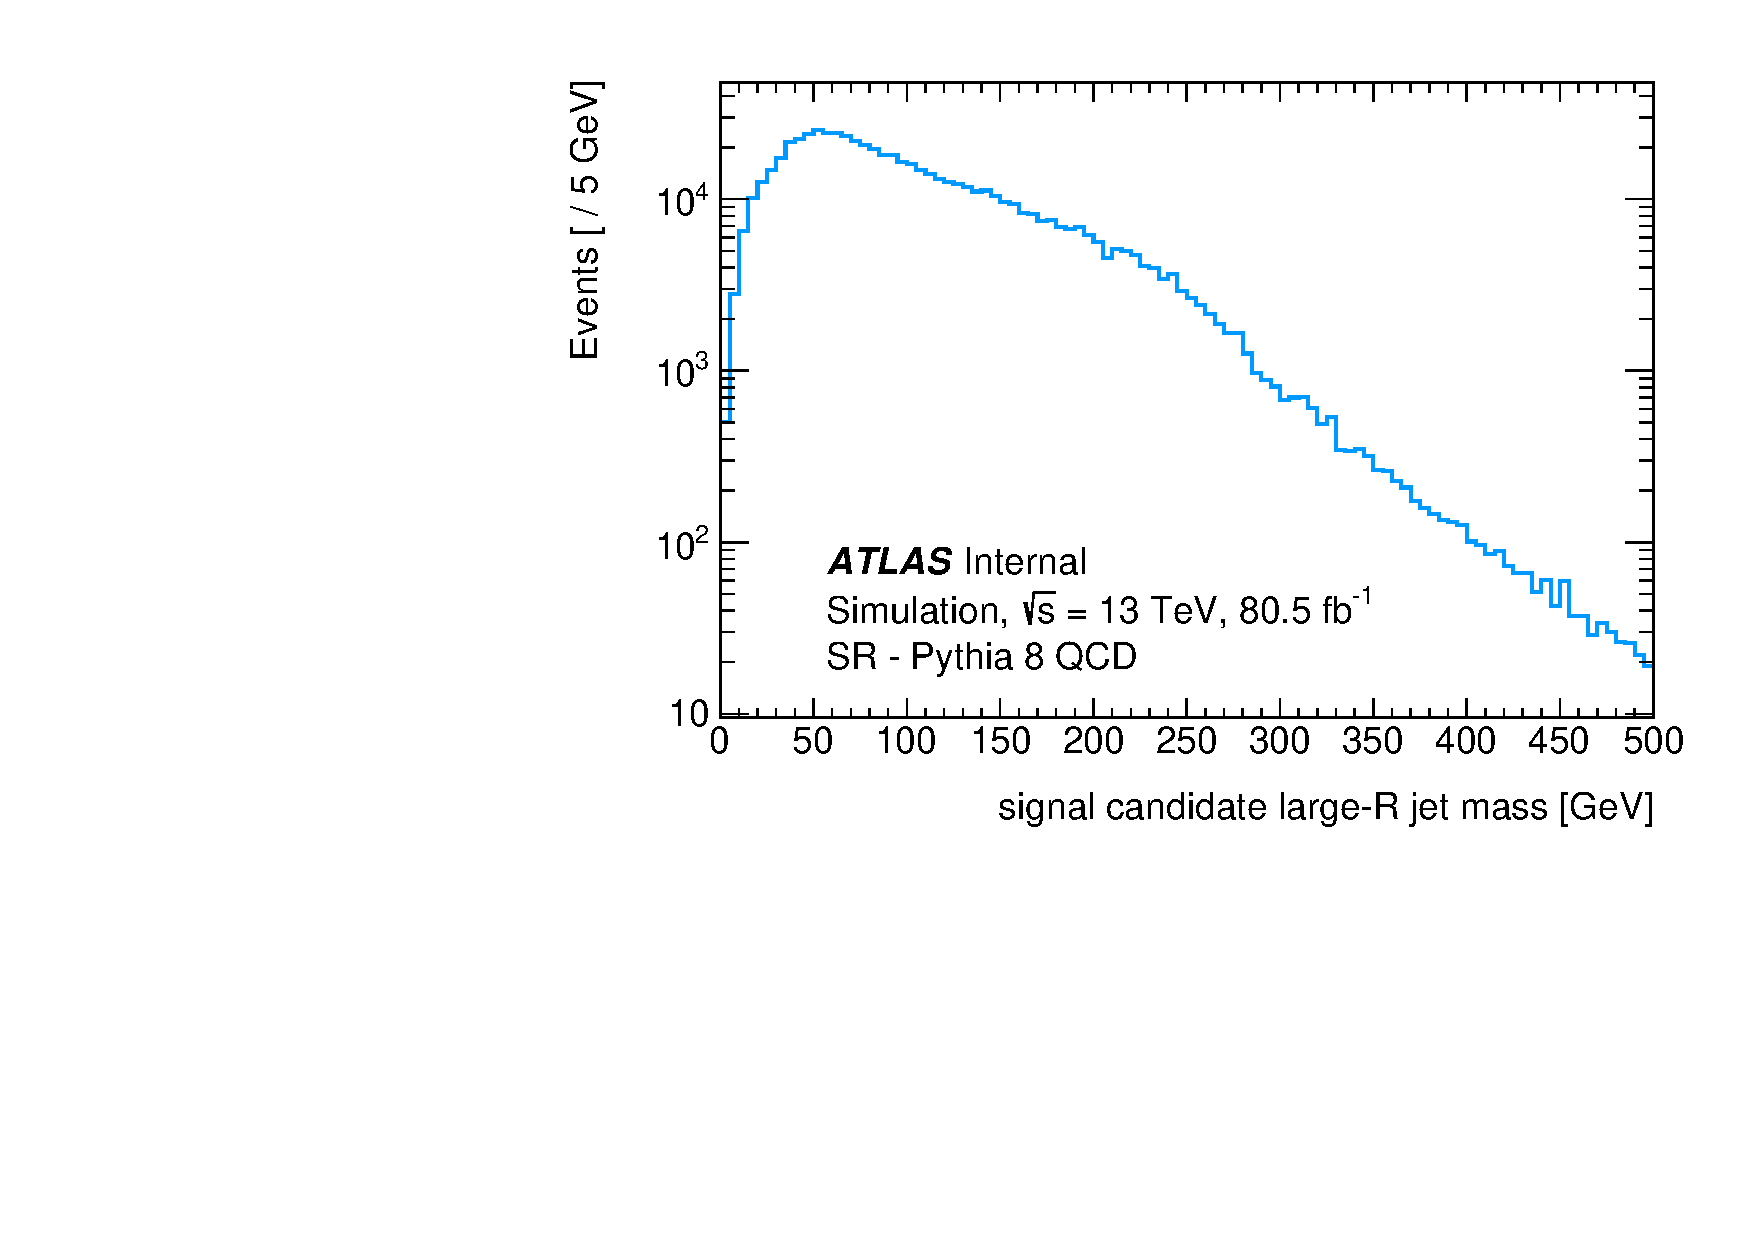
\includegraphics[width=0.49\linewidth]{figures/data/QCD_logy}} \hfill
  \subcaptionbox{Simulation of resonant $V$+jets and $t\bar{t}$ backgrounds in the signal region.  The Higgs simulation is included for comparison.}{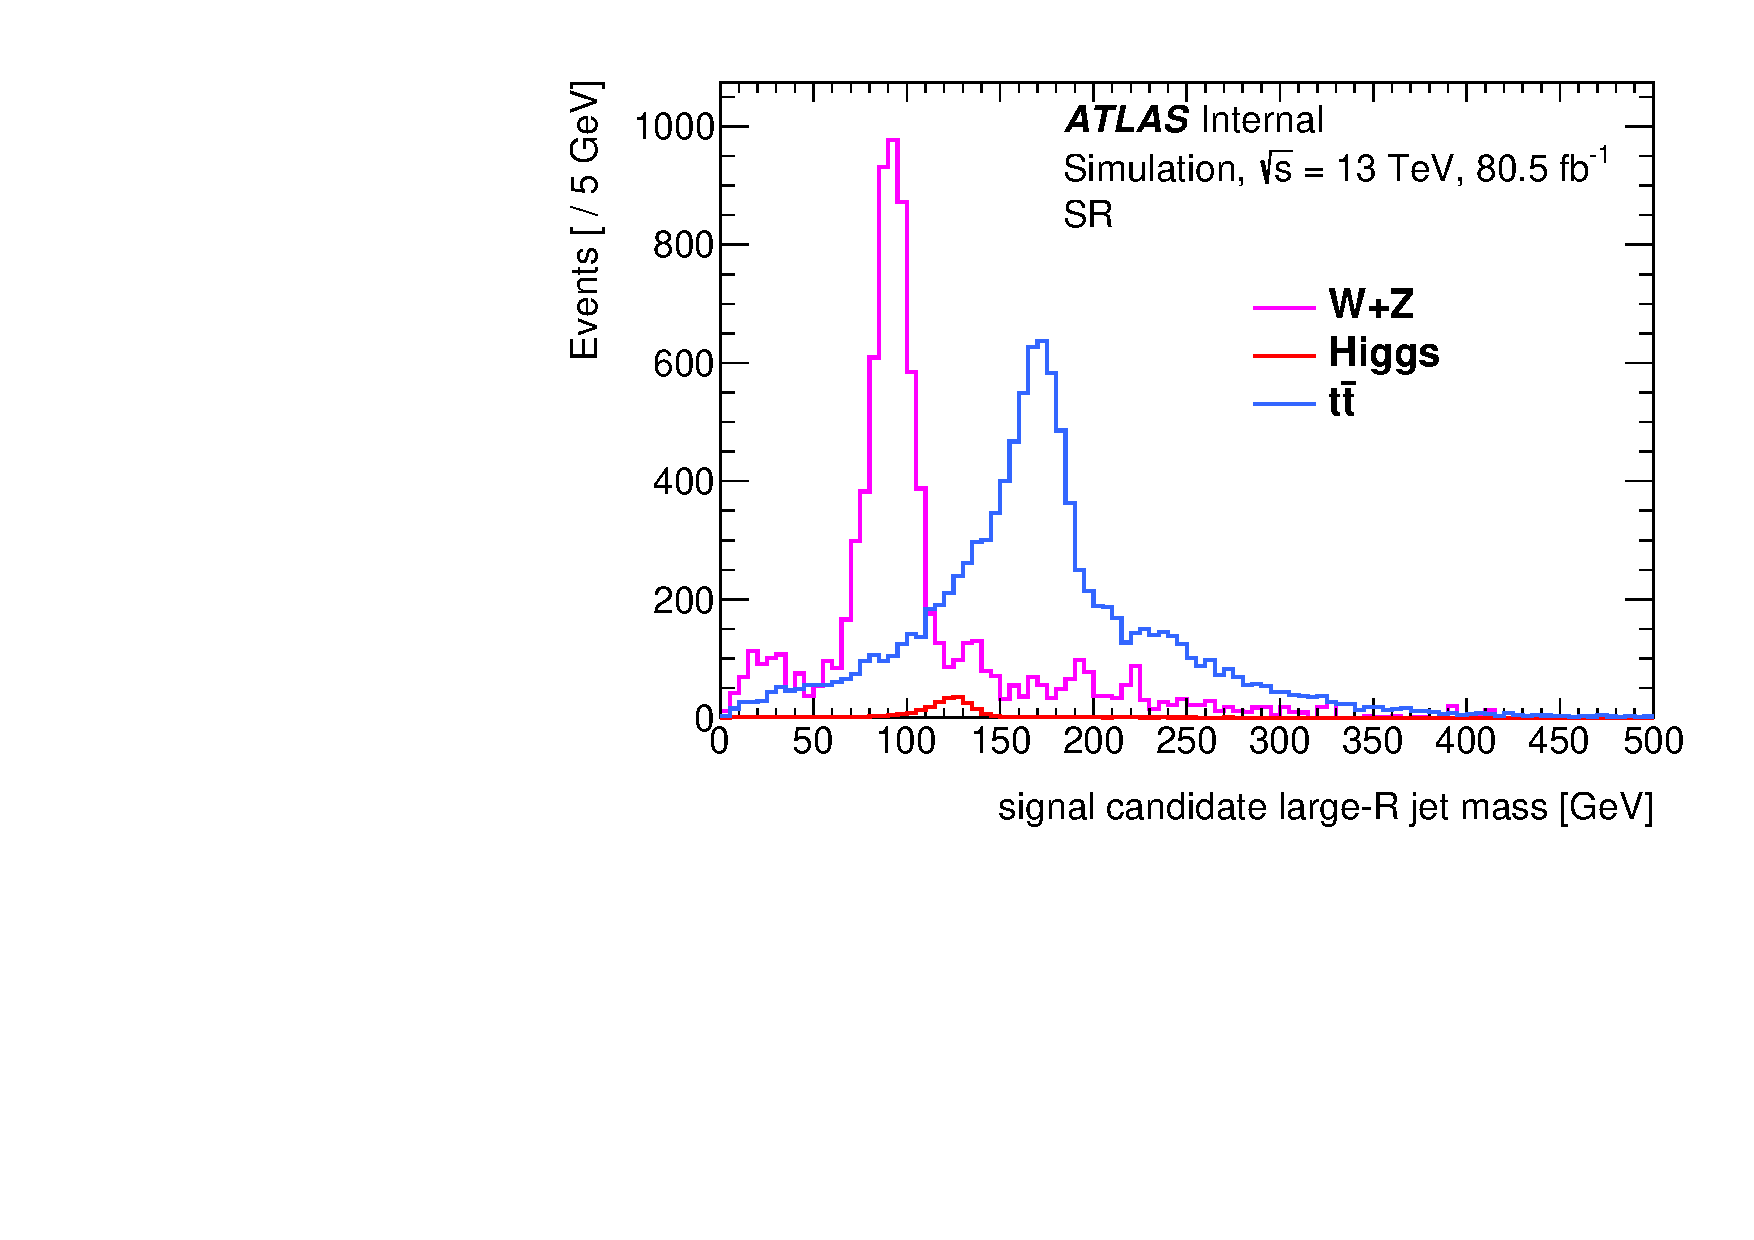
\includegraphics[width=0.49\linewidth]{figures/data/resonant_bkg}}
  \caption{Simulations of the non-resonant and resonant background contributions to the signal region for an integrated luminosity of $80.5~\ifb$}
  \label{simulated_background_shapes}
\end{figure}


\section{Hadronic Vector Boson Background} \label{sec:background:vqq}

The $V+\text{jets}$ template is constructed by fitting the generated MC
histogram with the sum of three Gaussians plus a constant term.  The systematic
variations, discussed in \Cref{chap:systematics}, of this template are re-fit
using the same functional choices.  This results in smooth histograms to be
used as input to the fit discussed in \Cref{chap:fit}.

\section{Top Quark Pair Background} \label{sec:background:ttbar}

The substantial contribution to the SR by boosted $t\bar{t}$ production shown
in \Cref{table:efficiencies_and_yields} makes its modeling a top
priority~\footnote{Pun!}.  Unfortunately, current MC generators are not able to
predict the $t\bar{t}$ cross section well in this boosted regime as seen in
\Cref{sec:background:mismodeling}.  This long-standing issue is likely due to
missing higher-order diagrams rather than due to suboptimal generator setup
\cite{ATL-PHYS-PUB-2018-009}.  To compensate for this mismodeling the
$t\bar{t}$ yield in the SR is corrected with a normalization scale factor.  The
scale factor, or $k$-factor, is derived by fitting the $t\bar{t}$ normalization
of the in the $t\bar{t}$ enriched control region ($\text{CR}_{t\bar{t}}$).  In
the final fit the SR $t\bar{t}$ MC sample is fit by a double-sided Crystal Ball
function \cite{Gaiser:1982yw} to smooth out statistical fluctuations, and then
its normalization is constrained with the derived flat $k$-factor using its
uncertainty.

\begin{figure}[!htbp]
\centering
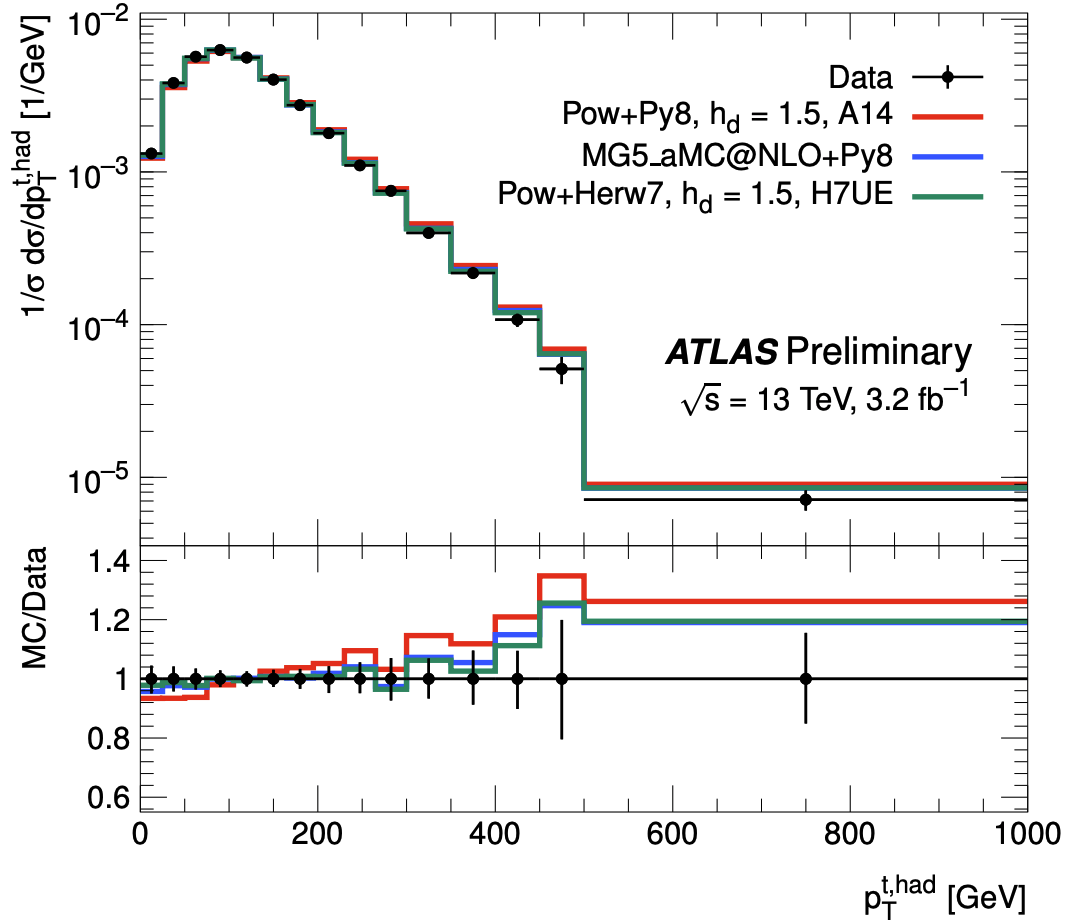
\includegraphics[width=0.6\linewidth]{figures/backgrounds/mismodeling}
\caption{Comparison in $\pT$ of the top quark for different generator setups
used to assess the NLO+PS matching as well as the parton shower and
hadronization uncertainty after optimization, compared to data at $\sqrt{s} =
13~\TeV$ \cite{ATL-PHYS-PUB-2018-009}.}
\label{sec:background:mismodeling}
\end{figure}

\subsection{Constructing the $\text{CR}_{t\bar{t}}$ Control Region}

The $t\bar{t}$-enriched control region uses the same $\pT$ selections as the
signal candidate large-$R$ jet in addition to the following criteria to select
$t\bar{t}$ events like the one shown in \Cref{sec:background:ttbar_depiction}.
Three regions are defined by requiring zero ($\text{CR}_{t\bar{t}0}$), one
($\text{CR}_{t\bar{t}}$) or two ($\text{CR}_{t\bar{t}2}$) tight quality
$b$-tags in the two leading VR track jets of the signal candidate. The
configuration with exactly one $b$-tag, $\text{CR}_{t\bar{t}}$, is was chosen
to exploit the single $b$-quark that results from the dominant decay mode of
the top quark $t \rightarrow bW$.  This one $b$-tag region has contributions from
$t\bar{t}$, single-top, $Z$ and $H$ when one $b$-tag is lost, and multijet when
the $b$-tag is faked.  The other two regions are used to validate the
extrapolation of the $k$-factor into the $\text{CR}_{\text{QCD}}$ and SR.

\begin{figure}[!htbp]
  \centering
\subcaptionbox{\label{sec:backgrounds:ttbar_feynman}}{
\resizebox{0.48\linewidth}{!}{
\begin{tikzpicture}
  \begin{feynman}
    % initial state particles
    \vertex (i1) {\(q\)};
    \vertex [below=2cm of i1] (i2) {\(q\)};

    % vertices
    \vertex [below right=1.cm and 1cm of i1] (a);
    \vertex [right=0.7cm of a] (b);

    % final state particles
    \vertex [above right=0.3cm and 0.5cm of b] (t1);
    \vertex [below right=0.3cm and 0.5cm of b] (t2);

    \vertex [above right=0.7cm and 0.7cm of t1] (W1);
    \vertex [blue, right=1.0cm of t1] (f1) {\(b\)};

    \vertex [blue, right=1.0cm of t2] (f2) {\(b\)};
    \vertex [below right=0.7cm and 0.7cm of t2] (W2);

    \vertex [above right=0.1cm and .6cm of W1] (f3) {\(\mu\)};
    \vertex [below right=0.1cm and .6cm of W1] (f4) {\(\nu_{\mu}\)};
    \vertex [above right=0.1cm and .6cm of W2] (f5) {\(q\)};
    \vertex [below right=0.1cm and .6cm of W2] (f6) {\(q\)};

    \diagram* {
      (i1) -- [fermion] (a) 
        -- [fermion] (i2),

      (a) -- [gluon, edge label'=\(g\)] (b),

      (t1) -- [orange, fermion, edge label'=\(t\)] (b)
        -- [orange, fermion, edge label'=\(t\)] (t2),

      (f1) -- [blue, fermion] (t1)
        -- [red, boson, edge label=\(W\)] (W1),
      (f2) -- [blue, fermion] (t2)
        -- [red, boson, edge label'=\(W\)] (W2),

      (f3) -- [fermion] (W1)
        -- [fermion] (f4),
      (f5) -- [fermion] (W2)
        -- [fermion] (f6),
    };

      
  \end{feynman}
\end{tikzpicture}
}} \hfill
\subcaptionbox{\label{sec:backgrounds:ttbar_cartoon}}{
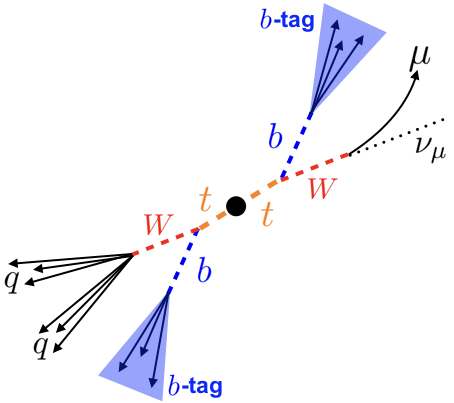
\includegraphics[width=0.48\linewidth]{figures/backgrounds/ttbar_cartoon}
}

\caption{(a) Feynman diagram of $t\bar{t}$ decay to $b$-quarks and leptonic $W$-boson decays. (b) Cartoon depicting $t\bar{t}$ decay to $b$-quarks and leptonic $W$-boson decays in center of mass frame.}
\label{sec:background:ttbar_depiction}

\end{figure}

To reduce multijet contamination in the sample the second top quark in the
opposite hemisphere of the signal candidate is required to decay leptonically
in the muon channel. \Cref{sec:backgrounds:phi_study} compares the $\Delta\phi$
between the leading muon in the event and the signal candidate jet for the
multijet and $t\bar{t}$ MC samples. This distribution shows the expected
back-to-back topology of the $t\bar{t}$ system depicted in
\Cref{sec:backgrounds:ttbar_cartoon} versus the multijet sample where the muons
come from the signal candidate due to hadron decays in flight. Thus, a cut of
$\Delta\phi(\text{muon} - \text{signal}) > \frac{2\pi}{3}$ was chosen to reduce
the QCD contribution by several orders of magnitude while only reducing the
$t\bar{t}$ contribution by roughly a factor of three~\footnote{This is expected
as the leptonic decay of $W$ is mostly agnostic to lepton flavor giving them
roughly uniform branching fractions, $BR(W \rightarrow \mu \nu_{\mu}) / BR(W
\rightarrow l \nu_l) = \frac{1}{3}$.  This is known as the universality of the
weak interaction}.

The QCD contribution is further suppressed by a cut on the muon $\pT$.
\Cref{sec:backgrounds:pt_study} compares the $\pT$ spectra for $t\bar{t}$ and
QCD before the $\Delta\phi$ cut selection. The larger mass of the $W$
boson leads to higher $\pT$ muons than the softer QCD-initiated muons.

\begin{figure}[!htbp]
\centering
\subcaptionbox{$\Delta \phi(\text{leading muon}-\text{signal})$ study \label{sec:backgrounds:phi_study}}{
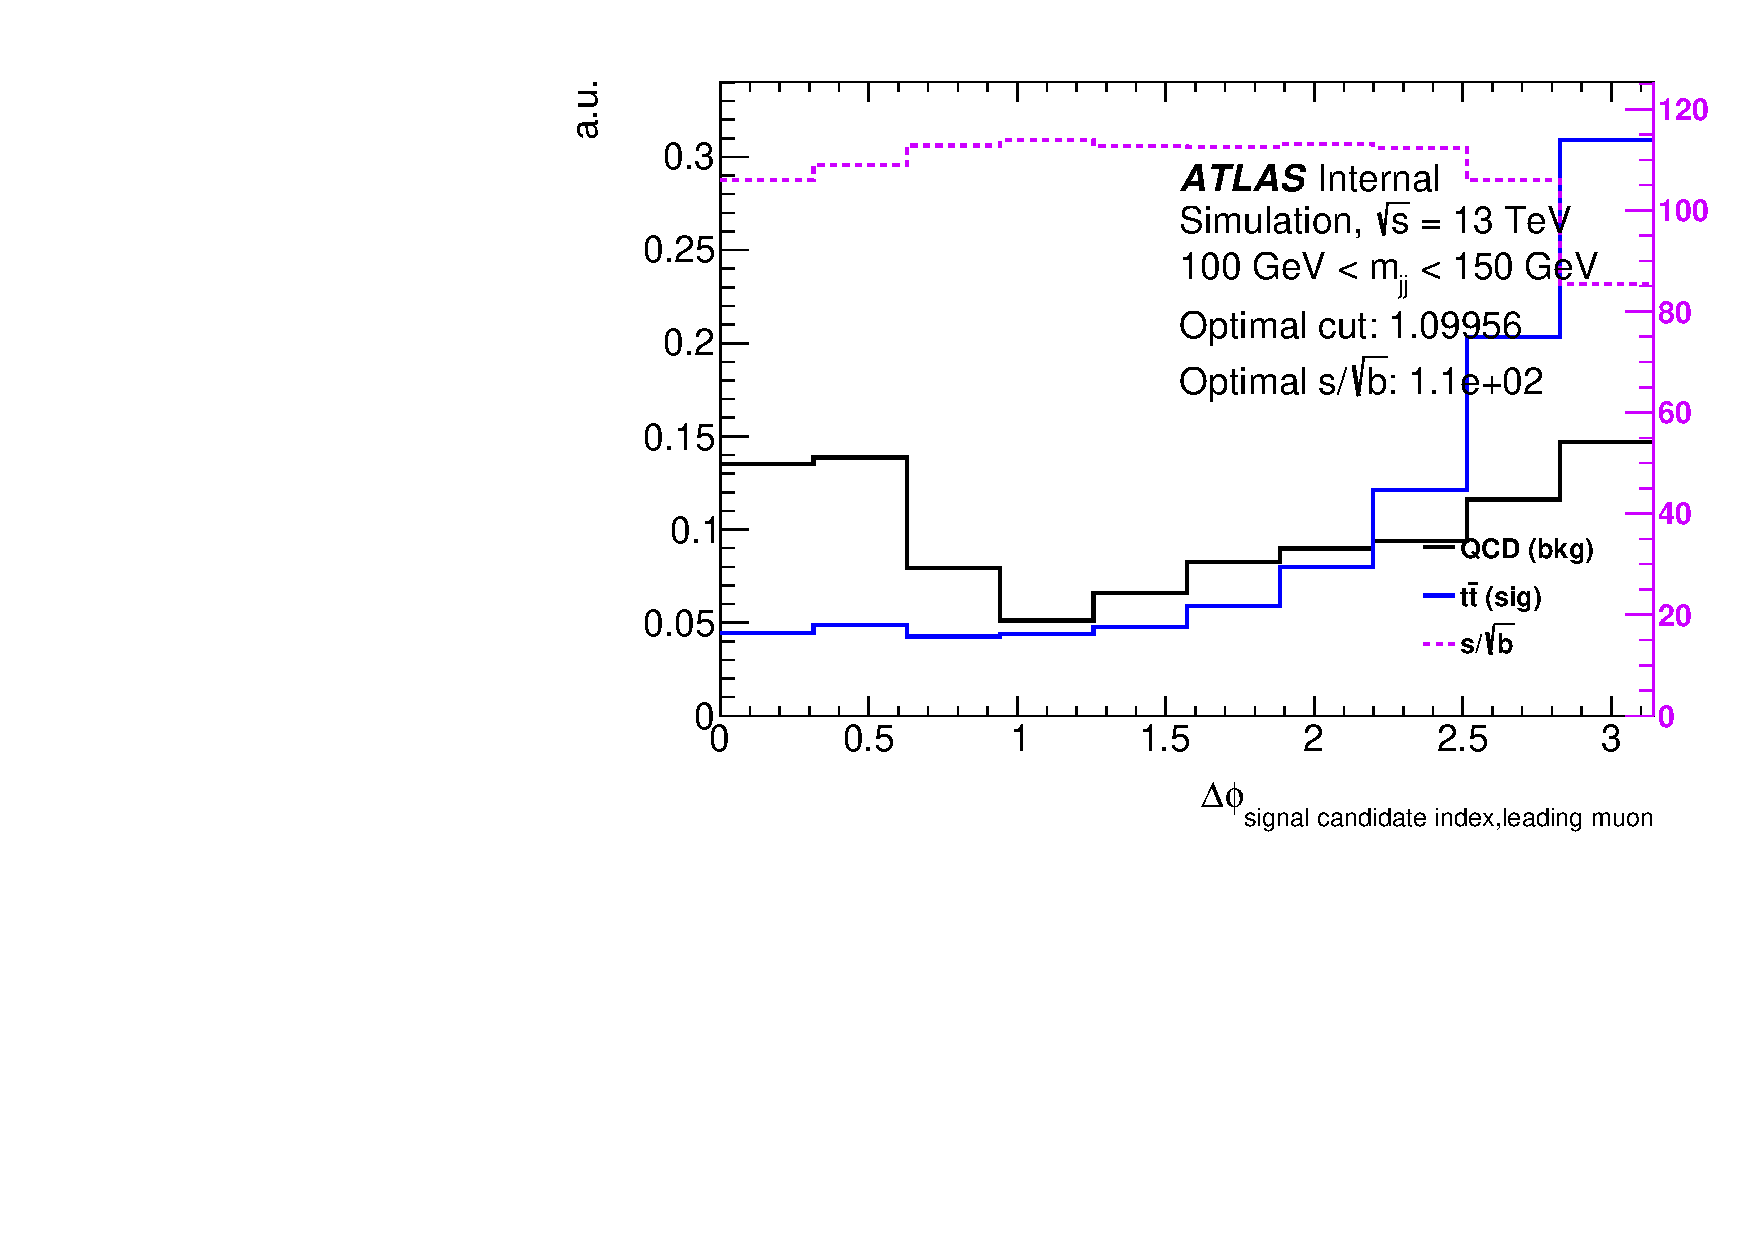
\includegraphics[width=0.48\linewidth]{figures/backgrounds/phi_study}
}\hfill
\subcaptionbox{Leading muon $\pT$ study \label{sec:backgrounds:pt_study}}{
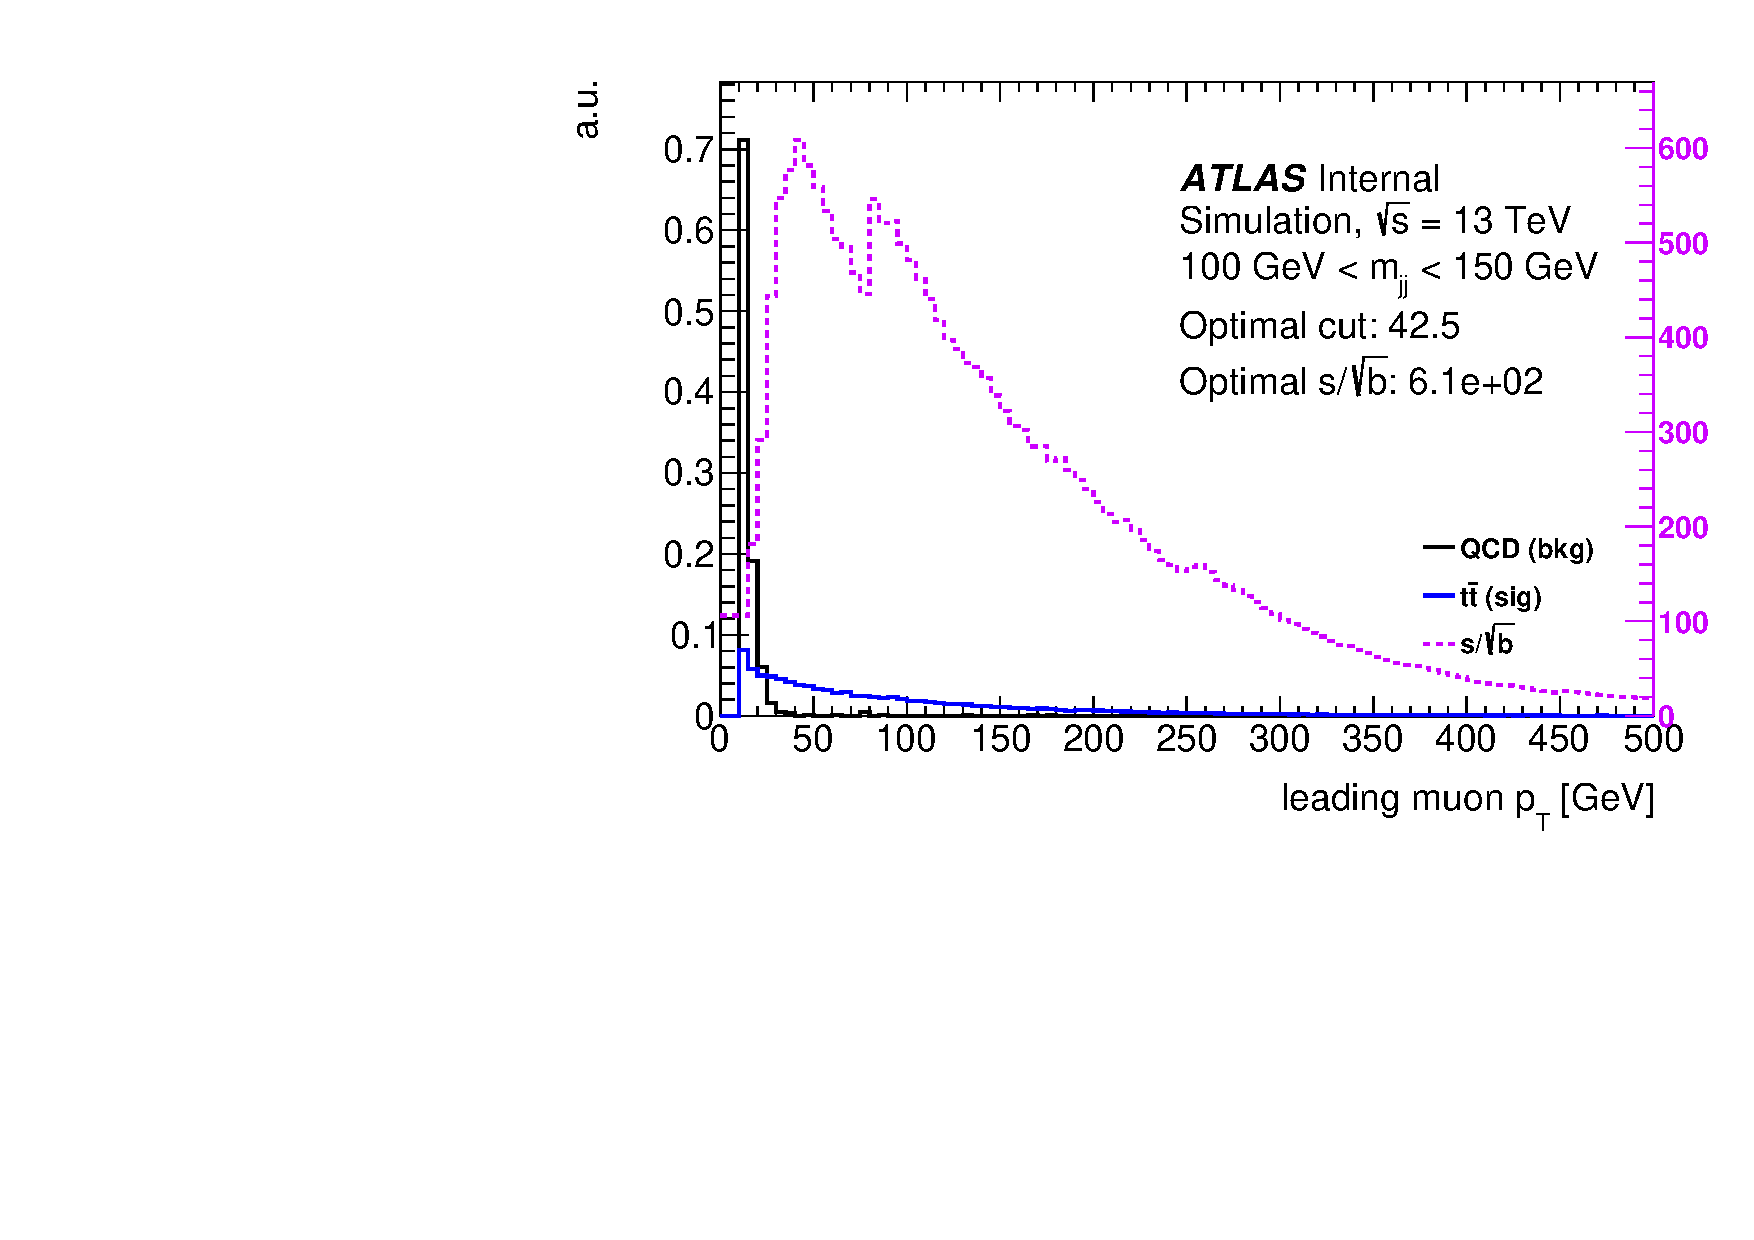
\includegraphics[width=0.48\linewidth]{figures/backgrounds/pt_study}
}
\caption{Comparison of the two variables, $\Delta \phi(\text{leading muon}-\text{signal})$ (a) and muon $\pT$ (b), between \textsc{Pythia}8 multijet and \textsc{Powheg} \ttbar simulated events used to create the \ttbar control region. The selection requires exactly one $b$-tagged track jet in the signal candidate \largeR jet. The magenta line shows the expected $s/\sqrt{b}$ significance with $80.5~\ifb$ \cite{Alison:2649017}.}
\label{sec:background:qcd_rejection_studies}
\end{figure}

Finally, at least one tight $b$-tagged track-jet is required to be within
$\Delta R < 1.5$ of the chosen muon.  This requirement exploits the collimation
of the decay products of the boosted top quark $t \rightarrow
b\mu\nu_{\mu}$.  This requirement reduces the contamination from $V(ll)$+jets
and $VV$ events. The above $\text{CR}_{t\bar{t}}$ requirements are summarized visually in \Cref{sec:background:ttbar_selection_diagram}.

\begin{figure}[!htbp]
\centering
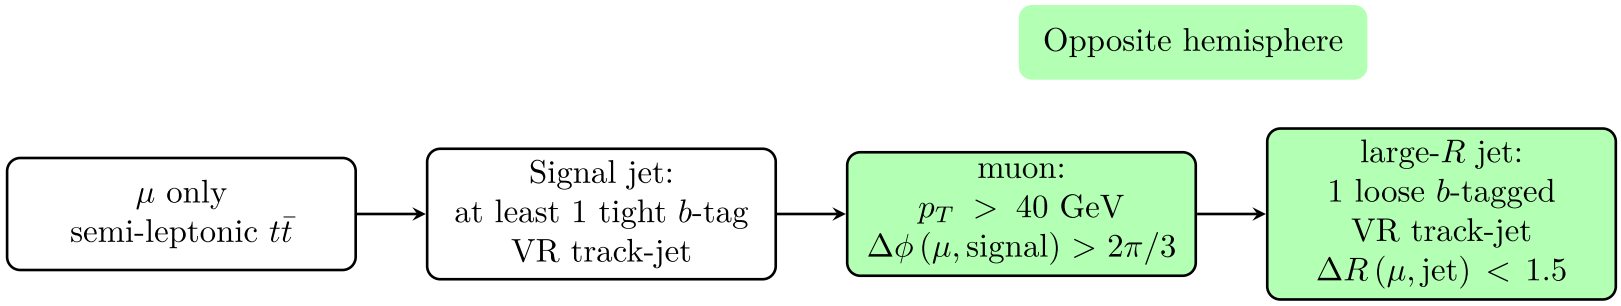
\includegraphics[width=1.0\linewidth]{figures/backgrounds/ttbar_selection}
\caption{Diagram of the $\text{CR}_{t\bar{t}}$ selection criteria \cite {Feickert:2690521}.}
\label{sec:background:ttbar_selection_diagram}
\end{figure}

\subsection{$k$-factor Estimation}

Finally the $t\bar{t}$ MC template is fit to the data in the
$\text{CR}_{t\bar{t}}$ over the mass range $100~\GeV$ to $200~\GeV$.  Single
top ($Wt$) and $W \rightarrow l\nu$ templates were included in the fit with
their normalizations kept constant. The full statistical and systematic
uncertainty is determined by running the Bayesian Analysis Toolkit (BAT)
\cite{Beaujean:2011zz}, discussed in \Cref{chap:fit}, with the large-$R$ jet
energy scale (JES), jet mass resolution (JMR), luminosity, $t\bar{t}$
modeling and flavor tagging systematic uncertainties discussed in
\Cref{chap:systematics}.

The pre- and post-fit distributions for the $\text{CR}_{t\bar{t}}$ are shown in
\Cref{sec:background:ttbar_fit} with the pull distributions shown in
\Cref{sec:background:ttbar_pulls}.  The JES and JMR systematics are constrained
by information about the peak in $t\bar{t}$ which was not available in the
dataset used to derive the recommendations. A $k$-factor of $0.84 \pm 0.11$ is
found for $\text{CR}_{t\bar{t}}$, showing that the MC overestimates the
$t\bar{t}$ yield as expected (see \Cref{sec:background:mismodeling}). This
value is used to constrain the $t\bar{t}$ contribution in the final fit to the
SR. The results for all three $t\bar{t}$ control regions are given in
\Cref{table:ttbar_kfactors}.  All three regions are consistent with eachoother
and the results of the dedicated boosted top quark study presented in reference
\cite{ATLAS:2016jct}.

\begin{table}
  \centering
  \caption{The \ttbar scale factors and their uncertainties from the three \ttbar
control regions. The value for CRttbar is used in the Signal Region. NOTE:
CRttbar2 fit failed due to low statistics but is almostly completely dominated
by ttbar in this region.  The value here is the simple ratio of number of events in ttbar
vs. data, and the uncertainty is the $t\bar{t}$ statistical uncertainty.}
  \begin{tabular}{@{}lrr@{}}
    \toprule
    Region & scale factor & uncertainty \\
    \midrule
    CRttbar0 & $0.87$ & $0.12$ \\
    CRttbar  & $0.84$ & $0.11$ \\
    CRttbar2 & $0.96$ & $0.21$ \\
    \bottomrule
  \end{tabular}
  \label{table:ttbar_kfactors}
\end{table}

\begin{figure}[!htbp]
\centering
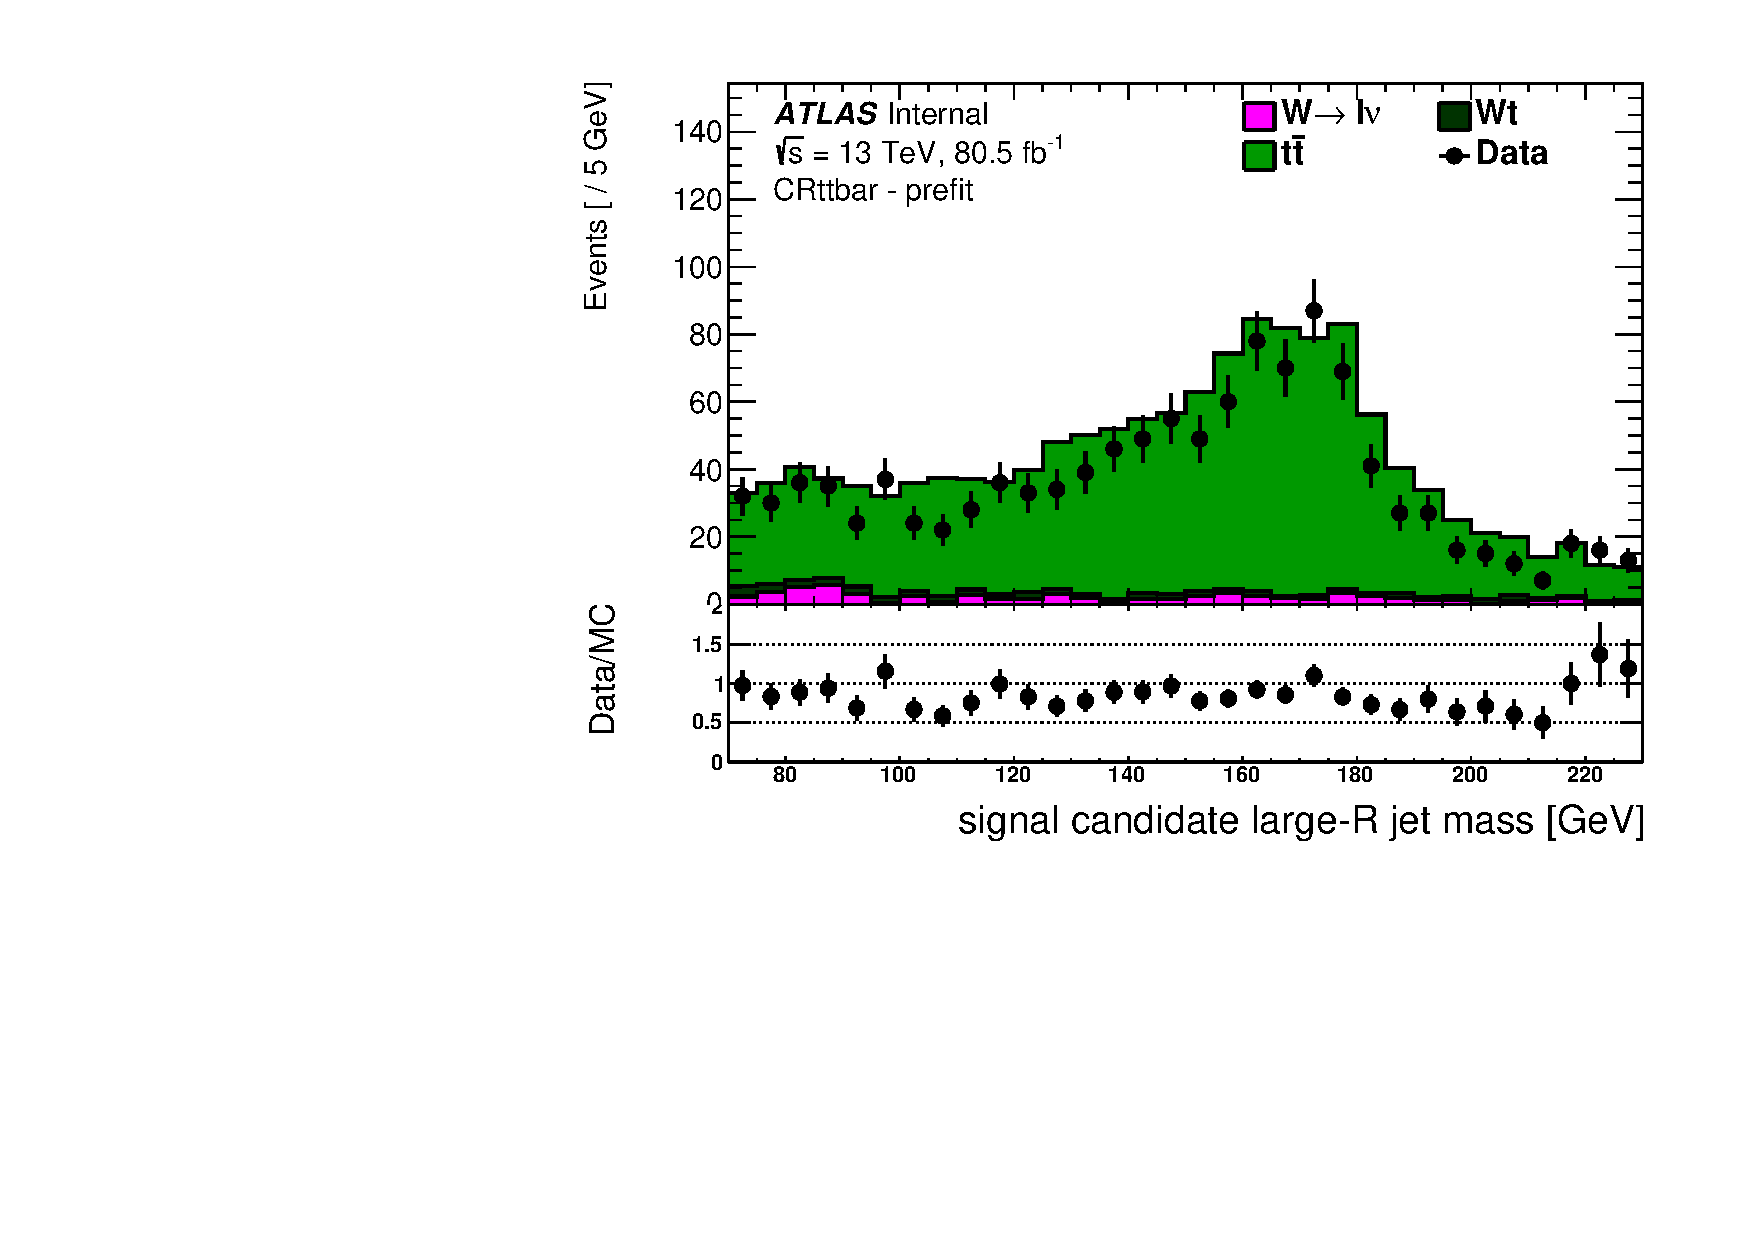
\includegraphics[width=0.49\linewidth]{figures/backgrounds/ttbar_prefit} \hfill
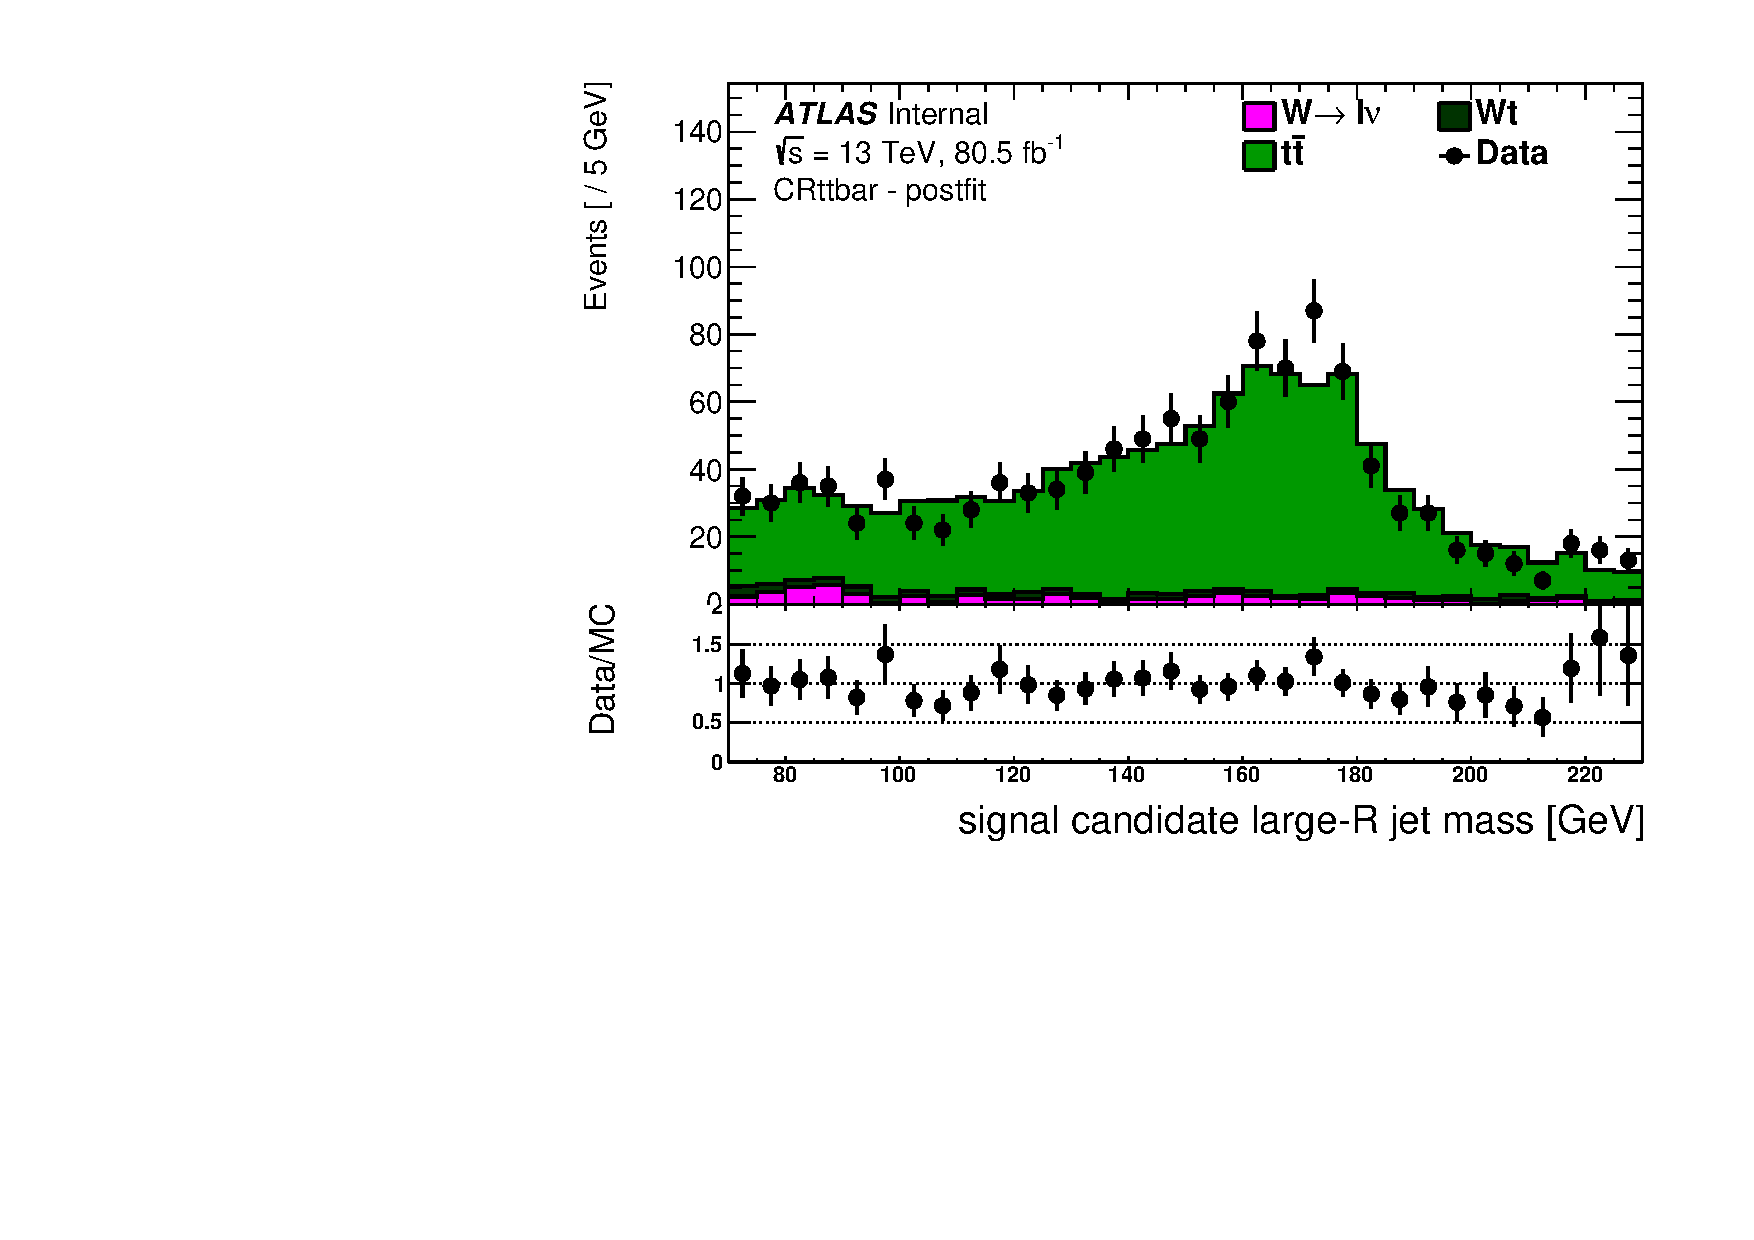
\includegraphics[width=0.49\linewidth]{figures/backgrounds/ttbar_postfit}
\caption{The pre-fit (left) and post-fit (right) data vs MC comparison for fitting the $\text{CR}_{t\bar{t}}$ region.}
\label{sec:background:ttbar_fit}
\end{figure}

\begin{figure}[!htbp]
\centering
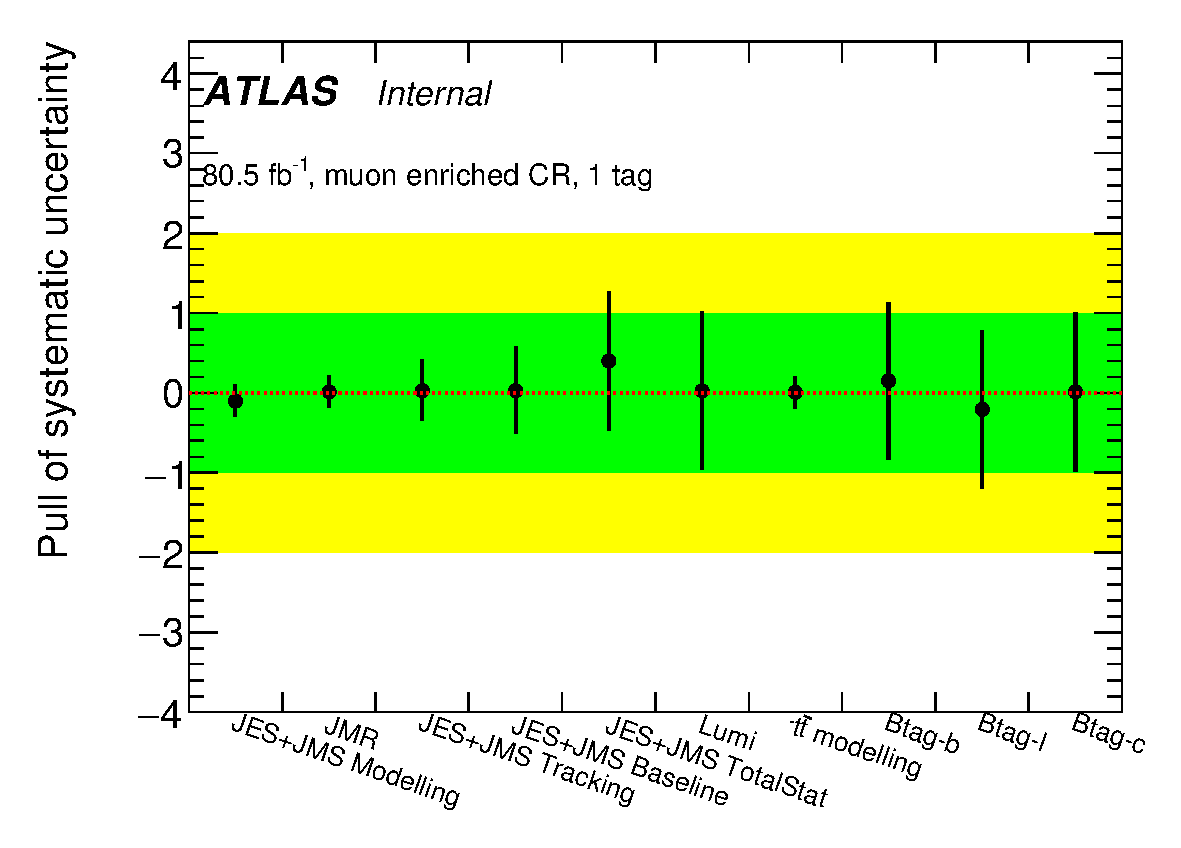
\includegraphics[width=0.7\linewidth]{figures/backgrounds/ttbar_pulls}
\caption{The pull distributions for the different nuisance parameters used in the $\text{CR}_{t\bar{t}}$ fit.}
\label{sec:background:ttbar_pulls}
\end{figure}

\section{Multijet QCD estimation} \label{sec:background:qcd}

The dominant background contribution to the SR comes from the non-resonant
multijet QCD process. Unfortunately the estimation of this process through MC
is not reliable due to the statistical precision of available samples and the
underlying inaccuracies of the event generation.  Thus, a data-driven estimate
was employed by fitting the large-$R$ jet mass distribution, $m_{J}$, in the SR
with a parametric function after validation of the procedure in the
$\text{CR}_{\text{QCD}}$.  This approach is further motivated by the good
agreement in shape of the $\text{CR}_{\text{QCD}}$ and SR over the mass range
of the fit, $70~\GeV$ to $230~\GeV$, as seen in
\Cref{fig:selection:sr_cr_shape}. A brief summary of this process is presented
below, with in-depth details available in Reference \cite{Feickert:2690521}.

The statistical precision of $\sim 1~\ifb$ of the
$\text{CR}_{\text{QCD}}$ is found to be comparable to that of the SR for a
luminosity of $80.5~\ifb$.  Thus, the $\text{CR}_{\text{QCD}}$ was
broken into 60 slices constructed using adjacent data runs resulting in an
average of $1.2~\ifb$ of data per slice.

Two families of parametric functions were used for this modeling.  The
polynomial exponential function was chosen to be the nominal model

\begin{equation}
\label{sec:background:polynomial}
f_{n} \left(x \middle|\,\vec{\theta}\right) = \theta_{0}\, \exp\left(\sum_{i=1}^{n} \theta_{i}\,x^{i}\right), \quad x = \frac{m_{J} - 150~\GeV}{80~\GeV},
\end{equation}

and the alternative model, the formal Laurent series,

\begin{equation}
\label{sec:background:laurent}
f_{n} \left(x \middle|\,\vec{\theta}\right) = a \sum_{i=0}^{n} \frac{\theta_{i}}{x^{i+1}}, \quad a=10^{5},\,x = \frac{m_{J} + 90~\GeV}{160~\GeV}.
\end{equation}

The $\theta$ coefficients are determined by the fit, $a$ is empirically chosen
to keep the scale of parameters at $\mathcal{O}(1)$, and the independent
variable $x$ parameterizes the fit range $m_{J}\in[70,230]$ GeV to $x\in[-1,1]$
for \Cref{sec:background:polynomial} and $x\in[1,2]$ for
\Cref{sec:background:laurent}.  This reparameterization was empirically seen to
provide improved numerical stability in the fit.

Both functions are tested on a random $\text{CR}_{\text{QCD}}$ slice to
determine the minimum number of model parameters needed to describe the shape
of the distribution.  The $Z$ + jets, $W$ + jets, and
$k$-factor corrected $t\bar{t}$ contributions are all scaled
by their cross sections times the luminosity and then subtracted from the slice
to remove bias from the fit.  The results of a likelihood ratio test with
Wilks' theorem \cite{wilks1938} and the $F$-test
\cite{snecdecor1991statistical} were both used to determine the minimum number
of model parameters for both function choices.  The Wilks test preferred a
five-parameter model for both while the $F$-test preferred a four-parameter
model for both.  To be conservative in our final estimate, the five-parameter
model was chosen for both the polynomial exponential function and the formal
Laurent series.

In order to determine the robustness of these fit functions, they were validated
using all of the $\text{CR}_{\text{QCD}}$ slices.  For these validation studies
the fit included properly scaled $Z$ + jets, $W$ + jets, $t\bar{t}$ and single
top contributions in addition to the $\text{CR}_{\text{QCD}}$ slice. Within the
statistical precision given by the different data slices, the $\chi^{2}/\text{ndf}$
from the individual fits is found to follow the expected distribution of a good
fit.

